\documentclass[tikz]{standalone}
\usepackage{tikz}
\usetikzlibrary{matrix,chains,positioning,decorations.pathreplacing,arrows}

\begin{document}

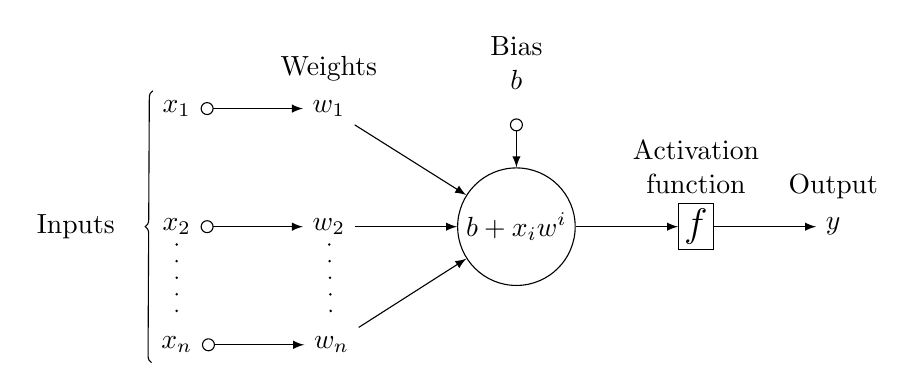
\begin{tikzpicture}[
	init/.style={
		draw,
		circle,
		inner sep=2pt,
		font=\normalsize,
		join = by -latex
	},
	squa/.style={
		draw,
		inner sep=2pt,
		font=\Large,
		join = by -latex
	},
	start chain=2,node distance=13mm
]

	\node[on chain=2] 
	  (x2) {$x_2$};
	
	\node[on chain=2,join=by o-latex] 
	  (w2) {$w_2$};
	
	\node[on chain=2,init] (sigma) 
		{$b + x_i w^i$};
	
	\node[on chain=2,squa,label=above:{\parbox{2cm}{\centering Activation \\ function}}]   
		{$f$};
	
	\node[on chain=2,label=above:Output,join=by -latex] 
		{$y$};
	
	\begin{scope}[start chain=1]
		\node[on chain=1] at (0,1.5cm) 
			(x1) {$x_1$};
		\node[on chain=1,label=above:Weights,join=by o-latex] 
			(w1) {$w_1$};
	\end{scope}
	
	\begin{scope}[start chain=n]
		\node[on chain=n] at (0,-1.5cm) 
			(xn) {$x_n$};
		\node[on chain=n,join=by o-latex] 
			(wn) {$w_n$};
	\end{scope}
	
	\node[label=above:\parbox{1cm}{\centering Bias \\ $b$}] at (sigma|-w1) (b) {};
	
	\draw[-latex] (w1) -- (sigma);
	\draw[-latex] (wn) -- (sigma);
	\draw[o-latex] (b) -- (sigma);
	
	\draw[line width=1pt, line cap=round, dash pattern=on 0pt off 6\pgflinewidth] (x2) -- (xn);
	\draw[line width=1pt, line cap=round, dash pattern=on 0pt off 6\pgflinewidth] (w2) -- (wn);
	
	\draw[decorate,decoration={brace,mirror}] (x1.north west) -- node[left=10pt] {Inputs} (xn.south west);
\end{tikzpicture}

\end{document}
